\subsection*{Fundamental: Decision-making in a Bureaucracy\label{sec:decision-making}}

Decisions are central to a bureaucratic organization. This book explores the topic of decisions, but decisions are not the only source of change in an organization. Occasionally events unfold without decisions being made either because the decision-makers are not informed or there is  \href{https://en.wikipedia.org/wiki/Willful_blindness}{intentional neglect}. 
\index{Wikipedia!willful blindness@\href{https://en.wikipedia.org/wiki/Willful_blindness}{willful blindness}}\iftoggle{WPinmargin}{\marginpar{$>$Wikipedia: Willful blindness}}{}
This book focuses on situations where bureaucrats recognize the need for a decision and want to make the best decision.

There are multiple types of decisions. 
A \gls{simple decision} \iftoggle{glossaryinmargin}{\marginpar{[Glossary]}}{}%
has one correct or beneficial choice and one or more wrong or harmful choices. The work of decision-making is then to gather information that identifies the correct or beneficial choice and select that option.

The best case scenario for any decision-making is one person making a well-informed, simple decision that has immediate consequence and the consequence is to the decision-maker. Examples from elementary school include arithmetic math problems, multiple-choice quizzes, spelling tests, and memorization tests. A bureaucrat's \href{https://en.wikipedia.org/wiki/Moral_injury}{moral injury}
\index{Wikipedia!moral injury@\href{https://en.wikipedia.org/wiki/Moral_injury}{moral injury}}\iftoggle{WPinmargin}{\marginpar{$>$Wikipedia: moral injury}}{}
(feelings of guilt, inadequacy, frustration)
comes from decision-making that involves multiple people, weak feedback loops with high latency, and complex decisions with multiple objectives. This last feature is the focus of the next section.
%A bureaucrat may not see the consequences of their actions. 

\subsubsection*{Example Decision Method: Pareto Frontier\label{sec:pareto}}

A complex decision may have many choices, and there may not be a best option. Which car should I buy? What food should I eat? Where should I live? What job should I have? There isn't  right outcome. There are formal techniques for navigating the process to arrive at a result. One approach for describing the situation is a \href{https://en.wikipedia.org/wiki/Pareto_front}{Pareto frontier}. 

The concept of a Pareto frontier is relevant when there are multiple possible solutions, no one of which is best. The set of adequate and not equivalent solutions is called the frontier. Some solutions are inadequate and are not part of the frontier. 
\index{Wikipedia!Pareto frontier@\href{https://en.wikipedia.org/wiki/Pareto_front}{Pareto frontier}}\iftoggle{WPinmargin}{\marginpar{$>$Wikipedia: Pareto frontier}}{}
If multiple solutions on a Pareto frontier exist then you can evaluate trade-offs. 

As an example of a complex decision made by one person with immediate consequence and direct relevance to the decision-maker, suppose you want to buy a car. You care about only two aspects: fuel efficiency and cost. See Figure~\ref{fig:pareto_frontier_cars} for an example of the Pareto frontier.

\begin{figure}[ht]
    \centering
    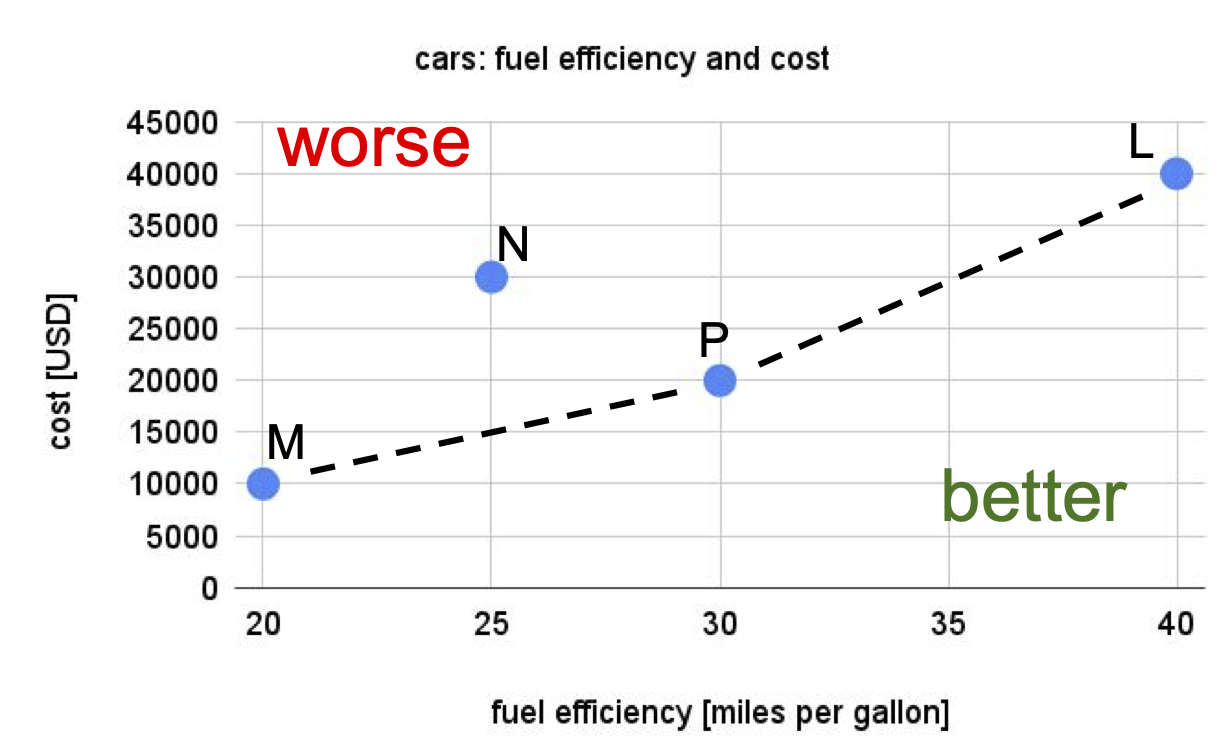
\includegraphics[width=1\textwidth]{images/pareto_frontier_car_options.pdf}
    \caption{Four cars: L, M, N, and P. The buyer's goal is to spend less money (lower on the vertical axis) and get better fuel efficiency (right on the horizontal axis). Choices not on the frontier should be avoided, but that doesn't yield a single result.}
    \label{fig:pareto_frontier_cars}
\end{figure}

Visualizing a Pareto frontier for two quantitative variables is easy, but typically decisions involve more factors. For example, evaluating the trade-off of three quantitative variables like 
passenger capacity, cost, and fuel efficiency creates a surface. With more than three variables visualization is less useful, though the analysis technique still applies. 

Another constraint on using Pareto frontier analysis is that it works well when there are many options relative to the number of variables you are optimizing for. 
The assessment does not work well when there are few choices relative to the number of variables. For example, suppose there are five choices of car and you want high fuel efficiency, sufficient cargo capacity, maximum number of passengers, stylish, low cost, low maintenance, good durability, and high resale value. Then defining a Pareto frontier is less helpful.

For a set of quantitative variables, a Pareto frontier does not account for the relative importance of different variables. Assigning weights to each of these factors merely stretches one axis relative to the other axes. 

There are many possible %decision-making 
% 2023-01-11: Brian Black says to remove redundancy
frameworks besides Pareto frontiers, but in practice a typical bureaucratic decision is ill-informed, has diffuse consequences, delayed impact, and does not affect the decision-maker. In bureaucratic processes there is rarely a formal assessment of options. 
Decisions are rarely recorded. 
Even afterward a decision can be difficult to evaluate for correctness because there are multiple stakeholders.

\textit{Tip}: If the people you want to convince are not swayed by data, then you can augment the \href{https://en.wikipedia.org/wiki/Cost\%E2\%80\%93benefit_analysis}{analysis of costs and benefits} with emotionally-impactful stories. 
\index{Wikipedia!cost-benefit analysis@\href{https://en.wikipedia.org/wiki/Cost\%E2\%80\%93benefit_analysis}{cost-benefit analysis}}
\iftoggle{WPinmargin}{\marginpar{$>$Wikipedia: cost-benefit analysis}}{}

\subsubsection*{Risks of Using Decision Frameworks}

%Decision-making 
% 2023-01-11: Brian Black says to remove redundancy
Frameworks can be attractive to bureaucrats intending to formalize 
\hyperref[sec:process]{processes} 
\marginpar{See page~\pageref{sec:process}.}%
%(see section~\ref{sec:process}) 
and encourage predictability, but there are potential risks to be aware of.  For example, analysis of costs and benefits can decrease the apparent responsibility of the decision-maker. Another risk is that cost-benefit analysis can be used to deflect criticism for an action. 

A good approach for data-driven quantitative analysis involves coming up with a testable hypothesis, pre-registering what actions are to be taken after assessing the results, then performing experiments and collecting data to evaluate the hypothesis. A decision can be characterized as quantitative when based on measurements. For example, before going into a store I set a threshold: I'm willing to spend up to \$30 on a pair of pants. If no pants that I want are available at or below that price then I don't buy pants. 

More commonly, a decision is made, then data is gathered that supports the desired outcome. Forming an opinion and then looking for evidence to back the outcome yields suboptimal results for the organization but maintains the relationships of the decision-maker. The value to the individual using that suboptimal approach is extracted from other members of the organization or subjects of the bureaucracy. 

% https://graphthinking.blogspot.com/2019/01/political-decisions-versus-science.html
To distinguish good data-driven decisions from the more common experiences let's be precise about the other ways decisions get made.
A decision is political when the basis is historical relationships, maintenance or creation of a relationship, or to enable future relationships. 
A decision is subjective when someone else faced with the same scenario would have come to a different conclusion. To avoid the appearance of subjective decision-making or political decision-making, a bureaucrat may frame a decision as ``data-driven." To evaluate which label is relevant, look for measurements and pre-registered actions. 
% https://graphthinking.blogspot.com/2018/06/data-driven-decisions-versus-data.html


Even when a bureaucrat is not intentionally biased towards an outcome, there are many ways to gather evidence -- informal conversations with stakeholders, formal surveys, measuring aspects of the problem. The choice of information gathering is constrained by cost and time, producing incomplete picture of the options. Poor data collection with biased sampling produces biased results. 

Even with valid and representative data measurement, decision-makers can be led astray by poor modeling. A model may use inapplicable techniques or may have implementation bugs.

For all the dangers described above,
%of decision-making methods, 
% 2023-01-11: Brian Black says to remove redundancy
there are worse approaches that do not rely on measurement. People rely on history (if they are aware of it) and perpetuate bad ideas, or take action based on what is best for their career, or decide based on how to accumulate more power, or choose based on what someone else says to do.  

%\subsubsection{Alternative Decision-Making Approaches}
% 2023-01-11: Brian Black says to remove redundancy
\subsubsection*{Alternative Approaches}
Identifying the spectrum of ways bureaucrats make decisions can decrease the surprise when you encounter the approaches in practice. 
\index{decrease surprise!decision-making techniques}
Enumerating the choices of how to make a decision allows for conversation about the pros and cons of each. The spectrum below is ordered from least effective to most effective and is not exhaustive.
\begin{enumerate}
    \item Random selection from the options (e.g., roll of the dice, shake the Magic 8 ball shown in Figure~\ref{fig:magic8ball}). The decision-maker is minimizing their involvement. 
    \item Rely on a hunch. The decision-maker is involved with the options but doesn't rely on data. 
    \item Rely on experience, whether yours or someone else's.
    \item Use a \href{https://en.wikipedia.org/wiki/Cost\%E2\%80\%93benefit_analysis}{cost-benefit model} that identified relevant factors and relates them to determine possible outcomes, 
    \index{Wikipedia!cost-benefit analysis@\href{https://en.wikipedia.org/wiki/Cost\%E2\%80\%93benefit_analysis}{cost-benefit analysis}}
    \iftoggle{WPinmargin}{\marginpar{$>$Wikipedia: cost-benefit analysis}}{} then gather data, and analyze to inform the decision.
    \item Make a hypothesis, design an experiment, carry out a test, collect data, and analyze.
\end{enumerate}

Brainstorming aspects of bureaucracy like ``How do decisions get made?" improves your emotional resilience when you encounter instances in your life. Building your Process Empathy involves thinking about how someone else might accomplish an activity. Not what is the best way, but what are all the possible ways. %Instead of cynicism and frustration, compassion and forgiveness. 

\begin{figure}
    \centering
    \includegraphics[width=0.4\textwidth]{images/magic8ball.pdf}
    \caption{Magic 8 ball for decision-making. The least effective method of selecting an option.}
    \label{fig:magic8ball}
\end{figure}

\subsubsection*{Why cost-benefit analysis models are not used}

Applying quantitative models to decision-making may seem a valuable path to optimal outcomes. Improved decision-making that helps stakeholders seems attractive. There are various reasons this approach is not taken. I outline the reasoning here not out of cynicism, but so that you can appropriately respond when confronted with arguments against \href{https://en.wikipedia.org/wiki/Cost\%E2\%80\%93benefit_analysis}{modeling costs and benefits}.\iftoggle{WPinmargin}{\marginpar{$>$Wikipedia: cost-benefit modeling}}{}
\index{Wikipedia!cost-benefit analysis@\href{https://en.wikipedia.org/wiki/Cost\%E2\%80\%93benefit_analysis}{cost-benefit analysis}}
\index{decrease surprise!reasons not to use cost-benefit modeling}%
Decreasing your surprise through the inoculation of exposure enables you to develop counterarguments. 

One reason to avoid cost-benefit modeling is that there is a lot of work to do, so coming up with a model is an \href{https://en.wikipedia.org/wiki/Opportunity_cost}{opportunity cost} -- you have less time available to do ``real work.'' 
\index{Wikipedia!opportunity cost@\href{https://en.wikipedia.org/wiki/Opportunity_cost}{opportunity cost}}\iftoggle{WPinmargin}{\marginpar{$>$Wikipedia: opportunity cost}}{}
Modeling every decision in detail is unrealistic, so triage is needed -- which decisions warrant what degree of investment in analysis. A person inexperienced in modeling decisions will take longer and is more likely to create a bad model. Practice designing models is expensive. Identifying relevant parameters for inclusion in a model is a learnable skill. 

If a person has a bad experience with cost-benefit modeling, they may be less likely to try again with other decisions. Bad experiences can come from using incorrect data, missing a critical variable, picking the wrong scope for a question, implementing the right model with the wrong math, misinterpreting the result, using a model that is too in-depth or not sufficiently deep, or failing to sell the result of an analysis to stakeholders.

Quantitative cost-benefit modeling doesn't account for personalities or organizational politics. The best options advocated for by a model may decrease the decision-maker's power or prestige, or harm relationships. 

A last reason why cost-benefit models are under utilized is the need for measurements. Designing good data collection and then collecting data is costly in terms of time and attention. Because the measurements involve people the data can get perverted by an undesired feedback loop. That concept is called \href{https://en.wikipedia.org/wiki/Campbell\%27s_law}{Campbell's law}. 
\index{Wikipedia!Campbell's law@\href{https://en.wikipedia.org/wiki/Campbell\%27s_law}{Campbell's law}}
\marginpar{$>>$ Folk Wisdom}
\index{folk wisdom!Campbell's law@\href{https://en.wikipedia.org/wiki/Campbell\%27s_law}{Campbell's law}}

\subsubsection*{Decision-Making Delay\label{sec:decision-delay}}

From an outsider's view, what appears as ``organizational inertia'' is the delay of internal decision-making and the delay of dissemination. 
Delay comes from:
\begin{itemize}
    \item Time used by each decision-maker to gather information, arrive at a decision, change processes, share their choice, and justify their choice. 
    %\item Forcing a continuous variable into a discrete set of choices. Typically the number of choices is small. Discrete choices for a continuous variable is a loss of effectiveness.
    % https://dynomight.net/teaching/
    \item Processes designed to detect and counter cheaters and people with malicious intent, whether that means a malicious bureaucrat or malicious subject. 
\item \href{https://en.wikipedia.org/wiki/Analysis_paralysis}{Analysis paralysis} 
\index{Wikipedia!analysis paralysis@\href{https://en.wikipedia.org/wiki/Analysis_paralysis}{analysis paralysis}}\iftoggle{WPinmargin}{\marginpar{$>$Wikipedia: Analysis paralysis}}{}
due to insufficient information or too much information. Another source  of paralysis is a lack of clarity about which framing is applicable.
\item When other people who are needed to carry out the action push back, either in disagreement or seeking clarification. If the impact on profit doesn't exist or is indirect, then justification for action isn't quantitatively obvious. Therefore there's a higher burden for communication.
\end{itemize}

Regardless of the source, delays for decisions are frustrating for stakeholders -- both the decision-makers and the subjects. Your Process Empathy is built on understanding the reason for why delays are expected.
% The following characterization has no consequence
% Decision-making by bureaucrats can be informal or formal, consensus-based or solo. 


\subsubsection*{A Bureaucratic Decision involves many Decisions}

\textit{What may appear a straightforward choice invokes related opportunities and constraints.}

A decision regarding shared resources is a collection of interdependent choices. After recognizing the need for a decision, follow-on decisions include identifying the stakeholders (who to include in an analysis) and identifying options. Who is a stakeholder and what options are available are interrelated. Involving more people expands the number of options and the complexity of coordination. Other choices associated with reducing uncertainty are how much time to spend on the decision, how much information to gather for the decision (see Dilemma~\ref{table:dilemma-personal-gather-data-lots-vs-little}),
\marginpar{See page~\pageref{table:dilemma-personal-gather-data-lots-vs-little}.}%
whether to make the decision or push the decision to someone with more expertise (see Dilemma~\ref{table:dilemma-personal-scope-of-speaking}), or whether to push the decision to someone with more exposure to the consequences.

Most decisions you make as a bureaucrat do not have hard deadlines. Instead, there are trade-offs in the allocation of your attention. Sooner is preferable since the consequence of the decision helps the organization and allows you to focus on other tasks, but delaying allows you to gather more information for a better-informed decision. See 
Dilemma~\ref{table:dilemma-personal-gather-data-lots-vs-little}
\marginpar{See page~\pageref{table:dilemma-personal-gather-data-lots-vs-little}.}%
and \hyperref[sec:dilemma-trilemma]{other related Dilemmas}.


If a bureaucrat relies on consulting an
\hyperref[sec:expertise]{expert},
\marginpar{See page~\pageref{sec:expertise}.}%
%(see section~\ref{sec:expertise} on expertise),
the decision-maker needs to be confident the expert is not  straying outside their area of expertise. For example, I don't rely on a botanist  to tell me how to change the oil in my car. 
Besides knowing their limitations, the expert should be clear about whether their input is a factual summary, a predictive assessment, or a value judgment. This complicates what you as a bureaucrat are interested in when deciding what's the best choice.


\subsubsection*{Transparency of Decision-Making\label{sec:transparency-of-decisions}}

\textit{A decision about decision-making is about what level of accessibility the decision should have before, during, and after the decision.}

% TODO: what's the prescription? This section just enumerates 

Your %decision-making 
% 2023-01-11: Brian Black says to decrease redundancy
process might change if made visible to stakeholders. You may provide more precise justifications or spend more time gathering evidence to support a claim. Strengthening the arguments is beneficial but takes time and resources. 

Frank conversations and exploratory brainstorming need protections to allow participants to be vulnerable. 
This is the motive for the \href{https://en.wikipedia.org/wiki/Chatham_House_Rule}{Chatham House Rule} -- meeting participants can use information from the discussion, but revealing who made a comment is not allowed.
\index{Wikipedia!Chatham House Rule@\href{https://en.wikipedia.org/wiki/Chatham_House_Rule}{Chatham House Rule}}\iftoggle{WPinmargin}{\marginpar{$>$Wikipedia: Chatham House Rule}}{}
The concept of transparency can apply before a decision is issued, while a policy is in effect, or after the consequence (as part of a review). 
Making decisions as part of a transparent process can make participants more risk-averse because of the potential for failure.

People affected by the decisions benefit from understanding how the decisions were made -- this is the reasoning behind  
\href{https://en.wikipedia.org/wiki/Government_in_the_Sunshine_Act}{Sunshine laws} and the 
\index{Wikipedia!Sunshine Act@\href{https://en.wikipedia.org/wiki/Government_in_the_Sunshine_Act}{Sunshine Act}}
\href{https://en.wikipedia.org/wiki/Freedom_of_Information_Act_(United_States)}{Freedom of Information Act (FOIA)}. 
\index{Wikipedia!Freedom of Information Act@\href{https://en.wikipedia.org/wiki/Freedom_of_Information_Act_(United_States)}{Freedom of Information Act}}\iftoggle{WPinmargin}{\marginpar{$>$Wikipedia: Freedom of Information Act}}{}
Even the symbolism of surveillance changes behavior~\cite{2005_Haley, 2007_Burnham}.



% TODO: TRANSITION to hierarchy

